\documentclass[12pt,conference,onecolumn]{IEEEtran}
\usepackage{diagbox}
\usepackage{graphicx}
\usepackage{amsmath}
\usepackage{amsfonts}
\usepackage{algpseudocode}
\usepackage{algorithm}
\usepackage{subfigure}
\usepackage{tikz}
% \usepackage[linesnumbered,ruled,vlined]{algorithm2e}
\usepackage{epsfig}
% \usepackage{pst-grad} % For gradients
% \usepackage{pst-plot} % For axes
\usepackage{cite}
\usetikzlibrary{shapes}
\usetikzlibrary{arrows,automata}
\usetikzlibrary{positioning}
\usetikzlibrary{patterns}
\usetikzlibrary{backgrounds}
\newtheorem{theorem}{Theorem}
\newtheorem{proof}{Proof}
\newtheorem{proposition}{Proposition}
\newtheorem{definition}{Definition}
\newtheorem{lemma}{Lemma}
\newtheorem{corollary}{Corollary}
\newtheorem{example}{Example}

%\renewcommand{\baselinestretch}{1}

\renewcommand{\ae}[1]{{\color{red}{#1}}}
\newcommand{\my}[1]{{\color{blue}{#1}}}
\newcommand{\old}[1]{{\color{green}{#1}}}
\begin{document}  
\title{Schedulability Analysis for Dual Priority Scheduling}  
\maketitle  


According to Baruah (2003, Dynamic- and Static-priority Scheduling of Recurring Real-time Tasks, Theorem~3), $\tau_i$ is schedulable on a single processor using static priority if and only if for each absolute deadline of a job  $d_{i,k}$ where $k\in N$, there exists an interval $d_{i,k-1}\leq t'\leq d_{i,k}$ for which the following condition holds:
\begin{equation}
dbf(\tau_i,t)+\sum_{\tau_j\in\{hp_i\}}rbf_i(\tau_j,t')\leq t'	
\end{equation} 

Here the demand bound function captures the maximum execution demand of $\tau_i$ for a time interval length $t$ if it is to meet all deadlines.
\begin{equation}
dbf(\tau_i,t)=\left(\lfloor \frac{t-D_i}{T_i}\rfloor+1\right)\times C_i
\end{equation} 


On the other hand, the request bound function  $rbf_i(\tau_j,t')$ denotes the maximum amount of time for which $\tau_j$ could \textbf{deny the processor} to lower priority task $\tau_i$ over some interval length of $t'$. \\\\



\section{Dual Priority}
Given a task system $\tau=\{\tau_1,\tau_2,\ldots, \tau_n\}$, we first make the following \textbf{assumptions}:
\begin{enumerate}
	\item Each task  $\tau_i$ has a original priority $n+i$ and a promotion priority $i$.
	\item Each task has a fixed promotion point $p_i$. The concerned job $J_{i,k}$ has its promotion point $P_i=r_{i,k}+p_i$.
\end{enumerate}

\my{Existing request bound function  $rbf_i(\tau_j,t')$  denotes the maximum cumulative execution requirement by jobs of $\tau_j$ by $t'$ that have ready times within any time interval of duration $t'$.  However this is not the case in dual priority scheduling as shown in the following example.}

\begin{example}
As shown in the Figure~1, when $r_i\leq t'\leq P_i$, the execution requirement of $J_{j,k}$ is $C_j$ because $\tau_i$  would execute only after $J_{j,k}$ finishes. However, when $P_i\leq t'\leq P_j$,  the time $J_{j,k}$ deny processor from $\tau_i$ is equal the time that $J_{j,k}$ has already executed, because $\tau_i$ has higher priority than $\tau_j$ during $[P_i,P_j]$.  This is a significantly different from the  static priority scheduling.
\begin{figure}[h!]
 \centering
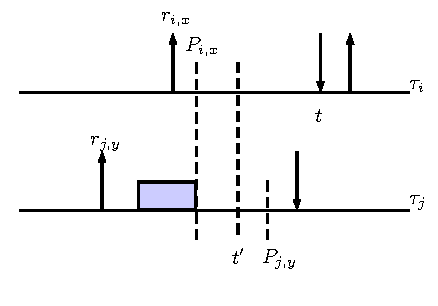
\includegraphics[scale=1]{Figure/E1}  
\caption{Example One}
  \label{fig:p3}
\end{figure}
\end{example}

Unfortunately, it is hard to calculate the exact time that  $J_{j,k}$  has executed, and therefore here instead,  we would use an upper bound of the resource $J_{i,k}$ has consumed to derive the test.

\begin{lemma}[Worst Case Pattern]
For each $\tau_j$, it can consume maximum resource during $[0,t']$, and hence $\tau_i$ can receive minimal resource by $t'$ if it is first released at $0$ and all jobs are released as soon as possible with period $T_i$. 
\end{lemma}
\begin{proof}
Suppose there is no deadline miss happens earlier, and as we shift the release pattern of $\tau_j$ left, $J_{j,1}$ will no longer request for any resource while the increment of the resource consumed by other jobs of $\tau_j$ is bounded by $C_j$. On the other hand, as we shift the pattern right, the promotion point of $J_{j,k}$  increases and hence $J_{j,k}$ is less likely to has higher priority than $\tau_i$ (and hence consume the resource).
\end{proof}




For dual priority scheduling, then we can have the following theorem.
\begin{theorem}
In dual priority scheduling, $\tau_i$ is schedulable on a single processor if and only if for each absolute deadline of a job  $d_{i,k}$ where $k\in N$, there exists an interval $r_{i,k}\leq t'\leq d_{i,k}$ for which the following condition holds:
\begin{equation}
\label{eq:1}
dbf(\tau_i,t)+\sum_{\tau_j\in\{\tau-\tau_j\}}rbf_i(\tau_j,t')\leq t'
\end{equation} 
where $rbf_i(\tau_j,t')$ upper bounds the resource that $\tau_j$ has consumed by $t'$ with corresponding priority and promotion point.
\end{theorem}
\begin{proof}
We can prove the statement that if $\tau_i$ is not schedulable then Equation~\ref{eq:1} would not hold. Suppose that $\tau_i$ is not schedulable then there are legal event sequences in which $\tau_i$ misses some deadline when $\tau_i$ is assigned with the current priority and promotion point. Let $S'$ denote such a sequence where $\tau_i$ misses deadline at the earliest time at $t$ (no deadline misses happens earlier).

It must be the cases that during $[0,t]$ some tasks are executing because otherwise the time interval between the last idle instant to $t$ could also construct such a sequence. Then it must be that during the time interval $[0,t']~(\forall t')$, other tasks have consumed an amount of resource more than 
\[
\sum_{\tau_j\in\{\tau-\tau_j\}}rbf_i(\tau_j,t')>t'-dbf(\tau_i,t)\Rightarrow dbf(\tau_i,t)>\max_{t'}(t'-\sum_{\tau_j\in\{\tau-\tau_j\}}rbf_i(\tau_j,t'))
\]
which contradicts the Equation~\ref{eq:1}.
\end{proof}







 
\begin{table}[h]
\caption{Notations}
\label{tab:x}
\large
\center
\begin{tabular}{|l|l|l|l|}
 \hline
 $n_j=\lfloor \frac{t'}{T_j}\rfloor$ & $r_j=n_j\times T_j$ &$P_j=n_j\times T_j+p_j$ \\
 \hline
$P_i=t-(D_i-p_i)$ & $r_i=P_i-p_i$ &$[a]_0=\max(a,0)$\\
 \hline
$n_j^s=\lfloor \frac{r_i}{T_j}\rfloor$  & $r_j^s=n_j^s\times T_j$& \\
 \hline
 $r_j^w=n_j^w\times T_j$ &	$n_j^w=\lfloor \frac{P_i}{T_j}\rfloor$ &	\\
  \hline
\end{tabular}
\end{table}

\section{Schedulability Test}
\begin{theorem}
A task system $\tau$ is schedulable by dual priority scheduling if the following hold:
\begin{equation}
\forall \tau_i\in \tau, t~\mbox{where }k\in\{1,2,\ldots\}: \exists t':
dbf(\tau_i,t)+\sum_{\tau_j\in\{\tau-\tau_j\}}rbf_i(\tau_j,t')\leq t'
\end{equation}
\end{theorem}

Here we also derive $rbf_{i}^1(\tau_j,t')$ which denotes \ae{maximum possible} execution that $\tau_j$ has received after $r_i$,  and $rbf_{i}^2(\tau_j,t')$ which denotes \ae{maximum possible} execution  that $\tau_j$ has received after $P_i$ (if $t'>P_i$).  Assuming no deadline miss happens earlier, the total execution before $r_i$ and $P_i$ should not exceed $r_i$ and $P_i$, respectively. As a result, we are able to tighten the schedulability test by bounding the total execution before $r_i$ and $P_i$ by $r_i$ and $P_i$, respectively.




\subsection{$rbf_i(\tau_j,t')$ when $j<i$}
\begin{figure}[h!]
 \centering
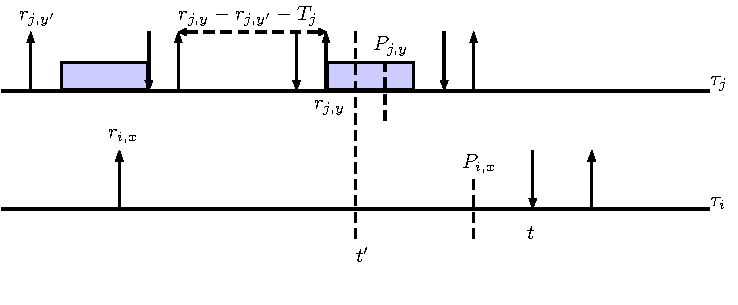
\includegraphics[scale=1]{Figure/C1}  
\caption{$ P_j\leq P_i$}
  \label{fig:case1}
\end{figure}
\textbf{Case 1 ( $P_j\leq P_i$)~as shown in  Figure~\ref{fig:case1}:} 

The promotion point of $P_i$ is greater than $P_j$, and hence $\tau_i$ always has lower priority than $\tau_i$. Thus its maximum possible execution units by $t'$ is 

	\begin{align*}
		rbf_i(\tau_j,t')=n_j.C_j +\min(C_j,t'-r_j)
	\end{align*}
Its maximum possible execution after $r_i$ is
	\begin{align*}
	\begin{split}
	rbf_{i}^1(\tau_j,t')=
	\begin{cases}
	\min\{C_j, t'-r_i\}&\mbox{if } r_j\leq r_i\\
	\min\{C_j, t'-r_j\}+\frac{r_j-r_j^s-T_j}{T_j}C_j+\min(C_j,[r_j^s+D_j-r_i]_0)  &\mbox{if } r_j>r_i
	\end{cases}
	\end{split}
	\end{align*}
Its maximum possible execution after $P_i$ is
	\begin{align*}
	\begin{split}
	rbf_{i}^2(\tau_j,t')=
	\begin{cases}
	\min\{C_j, [t'-P_i]_0\}&\mbox{if } r_j\leq P_i\\
	\min\{C_j, t'-r_j\}+\frac{r_j-r_j^w-T_j}{T_j}C_j+\min(C_j,[r_j^w+D_j-P_i]_0)  &\mbox{if } r_j>P_i
	\end{cases}
	\end{split}
	\end{align*}





\begin{figure}[h!]
 \centering
\includegraphics[scale=1]{Figure/C2}  
\caption{$P_j> P_i$}
  \label{fig:case2}
\end{figure}

\textbf{Case 2 ( $P_j> P_i$)~as shown in  Figure~\ref{fig:case2}} $\tau_i$ has higher priority than $\tau_j$'s last job during $[\max(r_j,P_i),P_j]$ if $P_i\leq P_j$:
	\begin{align*}
		rbf_i(\tau_j,t')=\lfloor \frac{t'}{T_j} \rfloor C_j +\min\left(C_j,t'-r_j-\left(\min\{t',P_j\}-\max\{r_j,P_i\}\right)\right)
	\end{align*}
Its maximum possible execution after $r_i$ is
\begin{align*}
\begin{split}
rbf_{i}^1(\tau_j,t')=
\begin{cases}
\min\{C_j,\min\{t',P_i\}-r_i\}&\mbox{if } t'<P_j\wedge r_j\leq r_i\\
\min\{C_j,\min\{t',\max(r_j,P_i)\}-r_j\} +\frac{r_j-r_j^s-T_j}{T_j}C_j &	\\+\min(C_j,[r_j^s+D_j-r_i]_0)&\mbox{if } t'<P_j\wedge r_j> r_i\\
\min\{C_j,t'-r_i-(P_j-P_i)\}&\mbox{if } t'\geq P_j\wedge r_j\leq r_i\\
\min\{C_j,t'-r_j-(P_j-\max(r_j,P_i))\}+\frac{r_j-r_j^s-T_j}{T_j}C_j&\\ +\min(C_j,[r_j^s+D_j-r_i]_0)&\mbox{if } t'\geq P_j\wedge r_j> r_i\\
\end{cases}
\end{split}
\end{align*}
Its maximum possible execution after $P_i$ is
\begin{align*}
\begin{split}
rbf_{i}^2(\tau_j,t')=
\begin{cases}
0&\mbox{if } t'<P_j \wedge r_j\leq P_i\\
\frac{r_j-r_j^w-T_j}{T_j}C_j+\min(C_j,[r_j^w+D_j-P_i]_0)&\mbox{if } t'<P_j \wedge r_j> P_i\\
\min\{t'-P_j,C_j\}&\mbox{if } t'\geq P_j \wedge  r_j\leq P_i\\
\min\{t'-P_j,C_j\}+\frac{r_j-r_j^w-T_j}{T_j}C_j+\min(C_j,[r_j^w+D_j-P_i]_0)&\mbox{if } t'\geq P_j \wedge  r_j> P_i\\
\end{cases}
\end{split}
\end{align*}


% %




\subsection{$rbf_i(\tau_j,t')$ when $j> i$}
 


\textbf{Case 1.1 ($P_i\leq P_j\wedge r_j\leq r_i$)~as shown in  Figure~\ref{fig:case3}}: $\tau_j$ may execute during $[r_j,r_i]$, and $\tau_j$ would not execute after $r_j$ or $P_i$ unless $\tau_i$ has finished.


% However we should assume all deadlines before $t'$ is meet. whether we should assume it is meet.
	\begin{figure}[h!]
 \centering
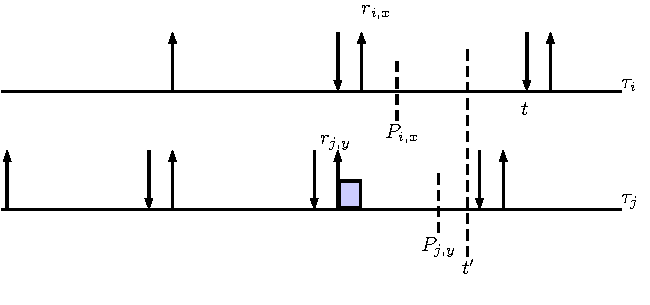
\includegraphics[scale=1]{Figure/C3}  
\caption{$P_i\leq P_j\wedge r_j\leq r_i$}
  \label{fig:case3}
\end{figure}
		\begin{align*}
		rbf_i(\tau_j,t')=(\lfloor \frac{t'}{T_j} \rfloor)\times C_j+\min(C_j,r_i-r_j)
	\end{align*}
\begin{align*}
\begin{split}
rbf_{i}^1(\tau_j,t')=rbf_{i}^2(\tau_j,t')=0
\end{split}
\end{align*}


\textbf{Case 1.2 ($P_i\leq P_j\wedge r_j> r_i$)~as shown in  Figure~\ref{fig:case4}}:  the last job of $\tau_j$ would not execute unless $\tau_i$ finishes. However all previous jobs are assumed to finish because otherwise the deadline miss should be already found. The $n_j-1$ job must already finish by $\min(P_i,r_j-T_j+D_j)$.

	\begin{figure}[h!]
 \centering
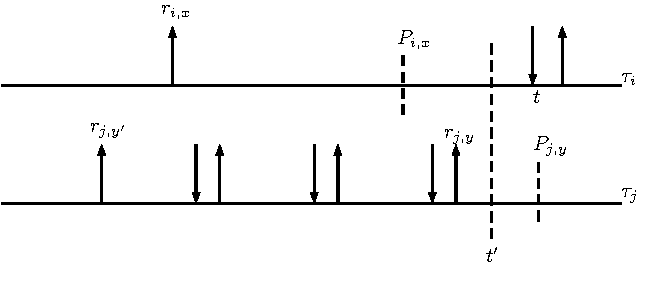
\includegraphics[scale=1]{Figure/C31}  
\caption{$P_i\leq P_j\wedge r_j> r_i$}
  \label{fig:case4}
\end{figure}

	\begin{align*}
		rbf_i(\tau_j,t')=(n_j)\times C_j
	\end{align*}
\begin{align*}
\begin{split}
rbf_{i}^1(\tau_j,t')&=\min(C_j, [\min(P_i,r_j-T_j+D_j)-r_i]_0)\\
rbf_{i}^2(\tau_j,t')&=0
\end{split}
\end{align*}

% \my{


\textbf{Case 2.1 ($P_i>P_j\wedge r_j\leq r_i$)~as shown in  Figure~\ref{fig:case5}}:the last job of $\tau_j$ can execute until $\min(t',P_i)$
	\begin{align*}
		rbf_i(\tau_j,t')=(n_j) C_j+\min\left(C_j,r_i-r_j+[\min(t',P_i)-\max(P_j,r_i)]_0\right)
	\end{align*}
	\begin{align*}
\begin{split}
rbf_{i}^1(\tau_j,t')=\min\{C_j,[\min(t',P_i)-\max(P_j,r_i)]_0\}
\end{split}
\end{align*}
\begin{align*}
\begin{split}
rbf_{i}^2(\tau_j,t')=0
\end{split}
\end{align*}

\begin{figure}[h!]
 \centering
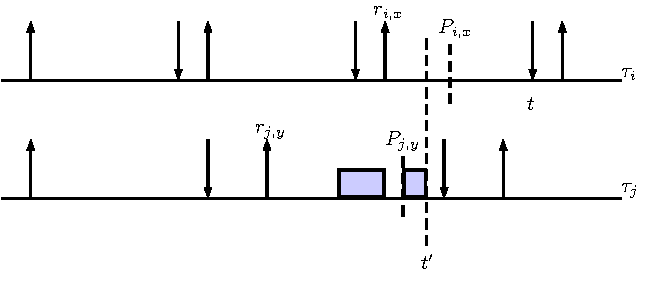
\includegraphics[scale=1]{Figure/C4}  
\caption{$P_i>P_j\wedge r_j\leq r_i$}
  \label{fig:case5}
\end{figure}

\begin{figure}[h!]
 \centering
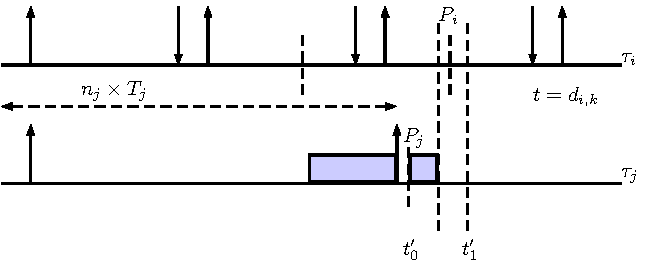
\includegraphics[scale=1]{Figure/C41}  
\caption{$P_i>P_j\wedge r_j> r_i $}
  \label{fig:case6}
\end{figure}

\textbf{Case 2.2 ($P_i>P_j\wedge r_j> r_i$)~as shown in  Figure~\ref{fig:case6}}: 
\begin{align*}
	rbf_i(\tau_j,t')=(n_j) C_j+\min\left(C_j,[\min(t',P_i)-P_j]_0\right)
\end{align*}


\begin{align*}
rbf_{i}^1(\tau_j,t')=\min\left(C_j,[\min(t',P_i)-P_j]_0\right)+\min(C_j,[r_j-T_j+D_j-r_i]_0)
\end{align*}

\begin{align*}
rbf_{i}^2(\tau_j,t')=0
\end{align*}





\section{Optimization Technique}
We can bound the total execution before $r_i$ or $P_i$ (if $t'>P_i$) by $r_i$ or $P_i$, respectively. For $\tau_i$ itself, we simply assume its execution demand after $r_i$ and $P_i$ is $C_j$.

\begin{equation}
F_1(\tau_i,t,t')=\min\left(r_i,n_i\times C_i+\sum_{\tau_j\in\{\tau-\tau_i\}}rbf_i(\tau_j,t')-rbf_{i}^1(\tau_j,t')\right)+\sum_{\tau_j\in\{\tau-\tau_i\}}rbf_{i}^1(\tau_j,t')+C_i
\end{equation}


\begin{equation}
F_2(\tau_i,t,t')=\min\left(P_i,n_i\times C_i+\sum_{\tau_j\in\{\tau-\tau_i\}}rbf_i(\tau_j,t')-rbf_{i}^2(\tau_j,t')\right)+\sum_{\tau_j\in\{\tau-\tau_i\}}rbf_{i}^2(\tau_j,t')+C_i
\end{equation}

\begin{equation}
\begin{split}
F(\tau_i,t,t')=
\begin{cases}
F_1(\tau_i,t,t')&\mbox{if } t'<=P_i\\
\min\{F_1(\tau_i,t,t'),F_2(\tau_i,t,t')\}&\mbox{otherwise}
	\end{cases}	
\end{split}
\end{equation}




We can derive a simple upper bound of $t$. Suppose that
\[
\forall~t'\in(k.T_i,k.T_i+D_i]:~F(\tau_i,t,t')>t'\Rightarrow\min_{t'\in(k.T_i,k.T_i+D_i]}\frac{F(\tau_i,t,t')}{t'}>1
\]
, and let
\[
H_i(t)=  U\times t+\sum_{\tau_j\in\{\tau-\tau_i\}}C_j\geq t\times u_i+(\lfloor \frac{t'}{T_j} \rfloor+1)C_j\geq F(\tau_i,t,t')
\]

then it must be that

\begin{align*}
\frac{H_i(t)}{t-D_i}>1\Rightarrow t-D_i< U\times t+\sum_{\tau_j\in\{\tau-\tau_i\}}C_j\Rightarrow t<\frac{D_i+\sum_{\tau_j\in\{\tau-\tau_i\}}C_j}{1-U}
	% &\mbox{Suppose there exists an t such that}~f_i(t_F,t')>t_F,~\mbox{it must be that}\\
	% &U\times t_F+\sum_{\tau_j\in\{\tau-\tau_i\}}C_j>t_F\Rightarrow t_F\leq \frac{\sum_{\tau_j\in\{\tau-\tau_i\}}C_j}{1-U}
\end{align*}

\section{Draft Simulation Results}

\begin{table}[h]
\caption{Notations}
\label{tab:x}
\large
\center
\begin{tabular}{|l|l|l|l|l|}
 \hline
Uniform Distribution&[0.88,0.9]&[0.93,0.95]&[0.95,0.97]&[0.97,0.99]\\
 \hline
Acceptance Ratio&1&1&0.995&0.982\\
 \hline
\end{tabular}
\end{table}
\end{document}  